\documentclass[12pt,a4paper]{article}

\usepackage[utf8]{vietnam}
\usepackage[vietnamese=nohyphenation]{hyphsubst}
\usepackage[vietnamese]{babel}
\usepackage[T1]{fontenc}
\usepackage{lmodern}
\usepackage{amsmath,amssymb}
\usepackage{graphicx}
\usepackage{booktabs}
\usepackage{tabularx}
\usepackage{array}
\usepackage{enumitem}
\usepackage{setspace}
\usepackage{xcolor}
\usepackage{float}
\usepackage{caption}
\usepackage{fancyhdr}
\usepackage{titlesec}
\usepackage[
  margin=2.2cm,
  top=2.4cm,
  bottom=2.4cm,
  headheight=14pt
]{geometry}
\usepackage{hyperref}
\DeclareUrlCommand\code{\urlstyle{tt}}
\setlength{\emergencystretch}{3em}

\hypersetup{
  colorlinks=true,
  linkcolor=black,
  urlcolor=blue!50!black,
  citecolor=black
}

\pagestyle{fancy}
\fancyhf{}
\fancyhead[L]{\small Topic Team --- DLinear \& NLinear}
\fancyhead[R]{\small WEEK01 Reading Note}
\fancyfoot[C]{\thepage}
\renewcommand{\headrulewidth}{0.4pt}

\titleformat{\section}{\large\bfseries}{\thesection.}{0.6em}{}
\titleformat{\subsection}{\normalsize\bfseries}{\thesubsection.}{0.5em}{}
\setlist[itemize]{leftmargin=1.4em, itemsep=0.25em, topsep=0.35em}
\onehalfspacing

% Cornell: Cue | Detail
\newcolumntype{C}{>{\raggedright\arraybackslash}p{0.26\textwidth}}
\newcolumntype{D}{>{\raggedright\arraybackslash}X}
\newcommand{\cornellhead}{%
  \toprule
  \textbf{Cue / Question} & \textbf{Detail} \\
  \midrule
}

\begin{document}

\begin{center}
  {\LARGE\bfseries Ghi chép đọc Paper}\\[0.35em]
  {\large LTSF-Linear: A Simple Strong Baseline for Long-Term Forecasts}\\[0.5em]
  {\normalsize Topic Team AIO2026 --- So sánh DLinear \& NLinear}\\[0.25em]
  {\small WEEK01 Reading Note --- Cornell (bảng); scan tay ở Phụ lục}
\end{center}

\vspace{0.5em}
\noindent\textbf{Nguồn:} Zeng et al., \textit{Are Transformers Effective for Time Series Forecasting?}
(LTSF-Linear / NLinear / DLinear).\\
\noindent\textbf{Mục tiêu note:} Hệ thống cơ chế Linear, NLinear, DLinear và liên hệ hướng regime-shift của nhóm.\\
\noindent\textbf{Scan tay gốc:} Phụ lục~\ref{app:cornell-scans}.

%% ====================================================================
\section{Bối cảnh LTSF}
%% ====================================================================

\begin{table}[H]
  \centering
  \caption{Cornell --- vấn đề chuỗi thời gian, LTSF, ý tưởng Linear / DLinear.}
  \label{tab:cornell-motivation}
  \small
  \begin{tabularx}{\textwidth}{@{}CD@{}}
    \cornellhead
    Vấn đề time series tài chính? &
    \textbf{Nhiễu:} ngay cả vùng biến động nhỏ, giá không đi đường thẳng mà dao động liên tục.                                                                                                                \\
                                  & \textbf{Không dừng (non-stationary):} thị trường đột ngột chuyển biến động nhỏ $\to$ lớn $\to$ phi tuyến.                                                                 \\
    \addlinespace
    Lợi nhuận + giá trị?          &
    Dự báo không chỉ \(t{+}1\) để có lời --- cần \textbf{nhìn xa} $\Rightarrow$ LTSF.                                                                                                                         \\
    \addlinespace
    Mô hình giải quyết được gì?
    Phụ thuộc dài hạn?            &
    \textbf{pattern} (tuần / tháng / năm),
    \textbf{seasonality} ($\sim$12 tháng),
    \textbf{market cycles} (3--5--10 năm).                                                                                                                                                                    \\
                                  & Mô hình truyền thống thường \textbf{fail to memorize + link} khoảng cách xa.                                                                                              \\
                                  & \textbf{Transformer:} Khó vì (1) temporal pattern rối (trend + season chồng), (2) self-attention point-wise / sparse vừa nặng vừa tận dụng thông tin kém trên chuỗi dài.. \\
    \addlinespace
    Giải pháp cần gì?             &
    Nhìn / kết nối điểm bất kể khoảng cách;
    tách tín hiệu dài hạn khỏi nhiễu cục bộ;
    rẻ hơn; tránh overfit.                                                                                                                                                                                    \\
    \addlinespace
    LTSF Linear / DLinear?        &
    \textbf{Linear:} ánh xạ tuyến tính cửa sổ lookback $\to$ tương lai (một ma trận \(W\)).                                                                                                                   \\
                                  & \textbf{DLinear:} \textbf{decomposition} trend + seasonality $\to$ 2 Linear rồi cộng.                                                                                     \\
    \bottomrule
  \end{tabularx}
\end{table}

\noindent\textit{Ghi chú TA / paper:} lập luận chính không còn là \(O(L^2)\) mà là
\textbf{mất thứ tự thời gian} (thí nghiệm xáo input).
Linear \(L\to T\) giữ được thứ tự vì trọng số phụ thuộc vị trí lookback.
Scan tay: Hình~\ref{fig:scan-motivation}.

%% ====================================================================
\section{Bài toán và chiến lược DMS}
%% ====================================================================

\begin{table}[H]
  \centering
  \caption{Cornell --- công thức tổng quát, recursive vs.\ direct, ba biến thể.}
  \label{tab:cornell-dms}
  \small
  \begin{tabularx}{\textwidth}{@{}CD@{}}
    \cornellhead
    NLinear (cont)?                  &
    \textbf{Chuẩn hóa / re-center} để giảm \textbf{distribution shift} trước khi Linear.                              \\
    \addlinespace
    Bài toán dự báo tổng quát        &
    \[
      \hat{y}_{t+1:t+H}
      = f\!\bigl(y_{t-L+1:t},\, x_{t-L+1:t},\, x_{t+1:t+H}^{s},\, s\bigr)+\varepsilon
    \]
    \(y\): lookback target; \(x\): support history;
    \(x^{s}\): support future (biết trước, vd.\ thứ trong tuần);
    \(s\): biến tĩnh; \(H\): horizon; \(L\): lookback.                                                                \\
    \addlinespace
    univariate / multivariate        &
    Một chuỗi vs.\ nhiều chuỗi / nhiều biến; output có thể là nhiều chuỗi.                                            \\
    \addlinespace
    Multistep: recursive vs.\ direct &
    \textbf{Recursive:} dự \(t{+}1\) rồi nhập lại $\Rightarrow$ \textbf{compounding error}.                           \\
                                     & \textbf{Direct (DMS):} ánh xạ thẳng \(L\to H\) --- Linear / NLinear / DLinear. \\
    \addlinespace
    Tóm tắt 3 biến thể               &
    Linear: một ánh xạ \(L\to T\).                                                                                    \\
                                     & DLinear: decomp trend+season $\to$ 2 linear.                                   \\
                                     & NLinear: normalize / trừ last $\to$ tránh lệch quá khứ vs.\ hiện tại.          \\
    \bottomrule
  \end{tabularx}
\end{table}

\noindent Scan tay: Hình~\ref{fig:scan-dms}.

%% ====================================================================
\section{LTSF-Linear \& NLinear}
%% ====================================================================

\begin{table}[H]
  \centering
  \caption{Cornell --- Linear (DMS/MSE) và NLinear (re-center + add last).}
  \label{tab:cornell-linear-nlinear}
  \small
  \begin{tabularx}{\textwidth}{@{}CD@{}}
    \cornellhead
    LTSF-Linear cơ chế?    &
    Linear reg trên cửa sổ \(L\) $\to$ output \(T\):
    \(\hat{y}=Wx+b\in\mathbb{R}^{T}\),
    \(W\in\mathbb{R}^{T\times L}\), \(b\in\mathbb{R}^{T}\), \(x\in\mathbb{R}^{L}\).                     \\
                           & Mỗi hàng \(W\) = một bước tương lai; \(W\) cố định với mọi \(x\) mới.      \\
    \addlinespace
    Loss / complexity      &
    DMS + MSE:
    \(\mathcal{L}=\frac{1}{B}\sum_n\bigl(\frac{1}{T}\sum_t(\hat{y}_t-y_t)^2\bigr)\).                    \\
                           & Param \(\approx LT\) (+ \(T\) bias); cost \(\propto BTL\).                 \\
    \addlinespace
    Channel-independent?   &
    Mặc định: từng biến riêng, \textbf{shared \(W\)}
    (trừ mode individual). Input \([B,L,C]\to[B,T,C]\).                                                 \\
    \addlinespace
    Hạn chế Linear?        &
    Phù hợp chuỗi ổn định; phi tuyến / đổi mặt bằng $\Rightarrow$ NLinear, DLinear.                     \\
    \addlinespace
    NLinear: sao trừ last? &
    \(x'=x-l\mathbf{1}\), \(\hat{y}'=Wx'+b\), \(\hat{y}=\hat{y}'+l\mathbf{1}\)
    (\(l\) = giá trị \textbf{cuối} lookback).                                                           \\
                           & Re-center: train quanh mức \(l\); additive level shift: cộng lại mặt bằng. \\
                           & Complexity \(\approx\) Linear.                                             \\
    \bottomrule
  \end{tabularx}
\end{table}

\noindent Scan tay: Hình~\ref{fig:scan-linear-nlinear}.

%% ====================================================================
\section{DLinear}
%% ====================================================================

\begin{table}[H]
  \centering
  \caption{Cornell --- DLinear (MA trend / residual), chọn \(m\).}
  \label{tab:cornell-dlinear}
  \small
  \begin{tabularx}{\textwidth}{@{}CD@{}}
    \cornellhead
    DLinear cơ chế? &
    Hai Linear trên \textbf{trend} + \textbf{seasonal}; output = tổng hai nhánh.                        \\
                    & Trend: \(\mathrm{MA}_m\) + padding.
    Vd.\ \([10,12,11,13]\), \(m{=}3\) $\to$ \([10.67,11,12,12.33]\).                                    \\
                    & Seasonal / residual: \(x - \mathrm{trend}\).
    Trend chậm; seasonal nhanh + chu kỳ.                                                                \\
    \addlinespace
    Công thức       &
    \(x_t=\mathrm{MA}_m(x),\; x_s=x-x_t\);
    \(\hat{y}_t=W_t x_t+b_t\), \(\hat{y}_s=W_s x_s+b_s\);
    \(\hat{y}=\hat{y}_t+\hat{y}_s\in\mathbb{R}^{T}\).                                                   \\
                    & Train: MSE--DMS như Linear. Param \(\approx 2(TL)+2T\); vẫn nhẹ vs.\ Transformer. \\
    \addlinespace
    Chọn \(m\)?     &
    \(m\) = low-pass / mức làm mượt.
    \(m\) lớn $\to$ mượt, mất chi tiết chu kỳ;
    \(m\) nhỏ $\to$ bám dao động ngắn.                                                                  \\
    \addlinespace
    So 3 model      &
    Linear: \(L\to T\) thẳng.
    NLinear: trừ last $\to$ Linear $\to$ cộng last.
    DLinear: MA + residual $\to$ 2 Linear $\to$ cộng.                                                   \\
    \bottomrule
  \end{tabularx}
\end{table}

\noindent Scan tay: Hình~\ref{fig:scan-dlinear}.

%% ====================================================================
\section{Background --- Autoformer}
%% ====================================================================

\begin{table}[H]
  \centering
  \caption{Cornell --- Autoformer (background cho DLinear).}
  \label{tab:cornell-autoformer}
  \small
  \begin{tabularx}{\textwidth}{@{}CD@{}}
    \cornellhead
    Vì sao đọc?       &
    Wu et al.\ NeurIPS 2021.
    DLinear mượn ý \textbf{decomp}; Autoformer làm \textbf{progressive} + Auto-Corr.              \\
    \addlinespace
    Bài toán          &
    LTSF horizon dài; pattern rối; attention point-wise/sparse tận dụng thông tin kém.            \\
    \addlinespace
    2 khối            &
    \textbf{SeriesDecomp:} \(T=\mathrm{MA}(X)\), \(S=X-T\)
    (trend-cyclical $\neq$ seasonal).                                                             \\
                      & \textbf{Auto-Corr:} \(R(\tau)=\sum_t X_t X_{t+\tau}\)
    (\(\tau\)=lag) $\to$ top-\(k\) $\to$
    \(w_\tau=\mathrm{Softmax}(R)\) $\to$
    \(\mathrm{agg}=\sum w_{\tau_k}\mathrm{Roll}(V,\tau_k)\).                                      \\
    \addlinespace
    1 bước layer      &
    \(\mathrm{agg}=\mathrm{AutoCorr}(\mathrm{input})\)
    $\to$ \(h=\mathrm{agg}+\mathrm{input}\)
    $\to$ \((S,T)=\mathrm{SeriesDecomp}(h)\).                                                     \\
                      & \(w_\tau\): softmax lag; \(W_{l,i}\): \textbf{learnable} projector trend. \\
    \addlinespace
    Encoder / Decoder &
    Enc.\ \#1: cả lookback \(X_{en}\); sau Decomp chỉ giữ \(S\).                                  \\
                      & Dec.\ init: \(X_{de}^{S}=[S_{\mathrm{recent}}\mid 0{\ldots}]\),
    \(X_{de}^{T}=[T_{\mathrm{recent}}\mid \bar{x}{\ldots}]\) (\(I/2+O\)).                         \\
                      & \(T\) chiếu bởi \(W\) \textbf{cộng dồn} \(T_{\mathrm{acc}}\);
    \(\hat{y}=S_{\mathrm{ref}}+T_{\mathrm{acc}}\).                                                \\
    \addlinespace
    vs.\ DLinear      &
    Autoformer: decomp nhiều lần + Auto-Corr.
    DLinear: decomp một lần + 2 linear.                                                           \\
    \bottomrule
  \end{tabularx}
\end{table}

%% ====================================================================
\section{So sánh nhanh \& hướng nhóm}
%% ====================================================================

\begin{center}
  \begin{tabular}{@{}llp{0.42\textwidth}@{}}
    \toprule
    \textbf{Mô hình} & \textbf{Ý chính}                      & \textbf{Khi nào hữu ích}      \\
    \midrule
    Linear           & Map \(L\to T\) trực tiếp (giữ thứ tự) & Chuỗi tương đối ổn / gần dừng \\
    NLinear          & Trừ \(l\) rồi cộng lại                & Distribution / level shift    \\
    DLinear          & Trend + seasonal + 2 Linear           & Có trend/season rõ            \\
    \bottomrule
  \end{tabular}
\end{center}

\vspace{0.5em}
\noindent Cả ba: \textbf{channel-independent + shared \(W\)} theo mặc định paper.\\[0.35em]
\noindent Theo outline Topic Team: reproduce baseline trên VIC và thử \textbf{regime shift}
(đổi phân bố / trend--seasonality giữa train--test) để xem NLinear vs.\ DLinear bền bao nhiêu.

\section*{Tài liệu}
\begin{itemize}
  \item Zeng, A., Chen, M., Zhang, L., \& Xu, Q.
        \textit{Are Transformers Effective for Time Series Forecasting?}
        (LTSF-Linear / NLinear / DLinear).
  \item Wu, H., Xu, J., Wang, J., \& Long, M.
        \textit{Autoformer: Decomposition Transformers with Auto-Correlation
          for Long-Term Series Forecasting} (NeurIPS 2021).
  \item Cornell handwritten scans --- Phụ lục~\ref{app:cornell-scans}; file gốc \code{Figures/}.
  \item Outline nhóm: \code{Working_Files/WEEK01_Outline.md}.
  \item Góp ý TA: lập luận chính = mất thứ tự thời gian (thí nghiệm xáo input);
        channel-independent + shared weights khi cài đặt.
\end{itemize}

%% ====================================================================
\appendix
\section{Scan Cornell notes gốc}
\label{app:cornell-scans}
%% ====================================================================
\noindent Đối chiếu với các bảng~\ref{tab:cornell-motivation}--\ref{tab:cornell-dlinear}.

\begin{figure}[H]
  \centering
  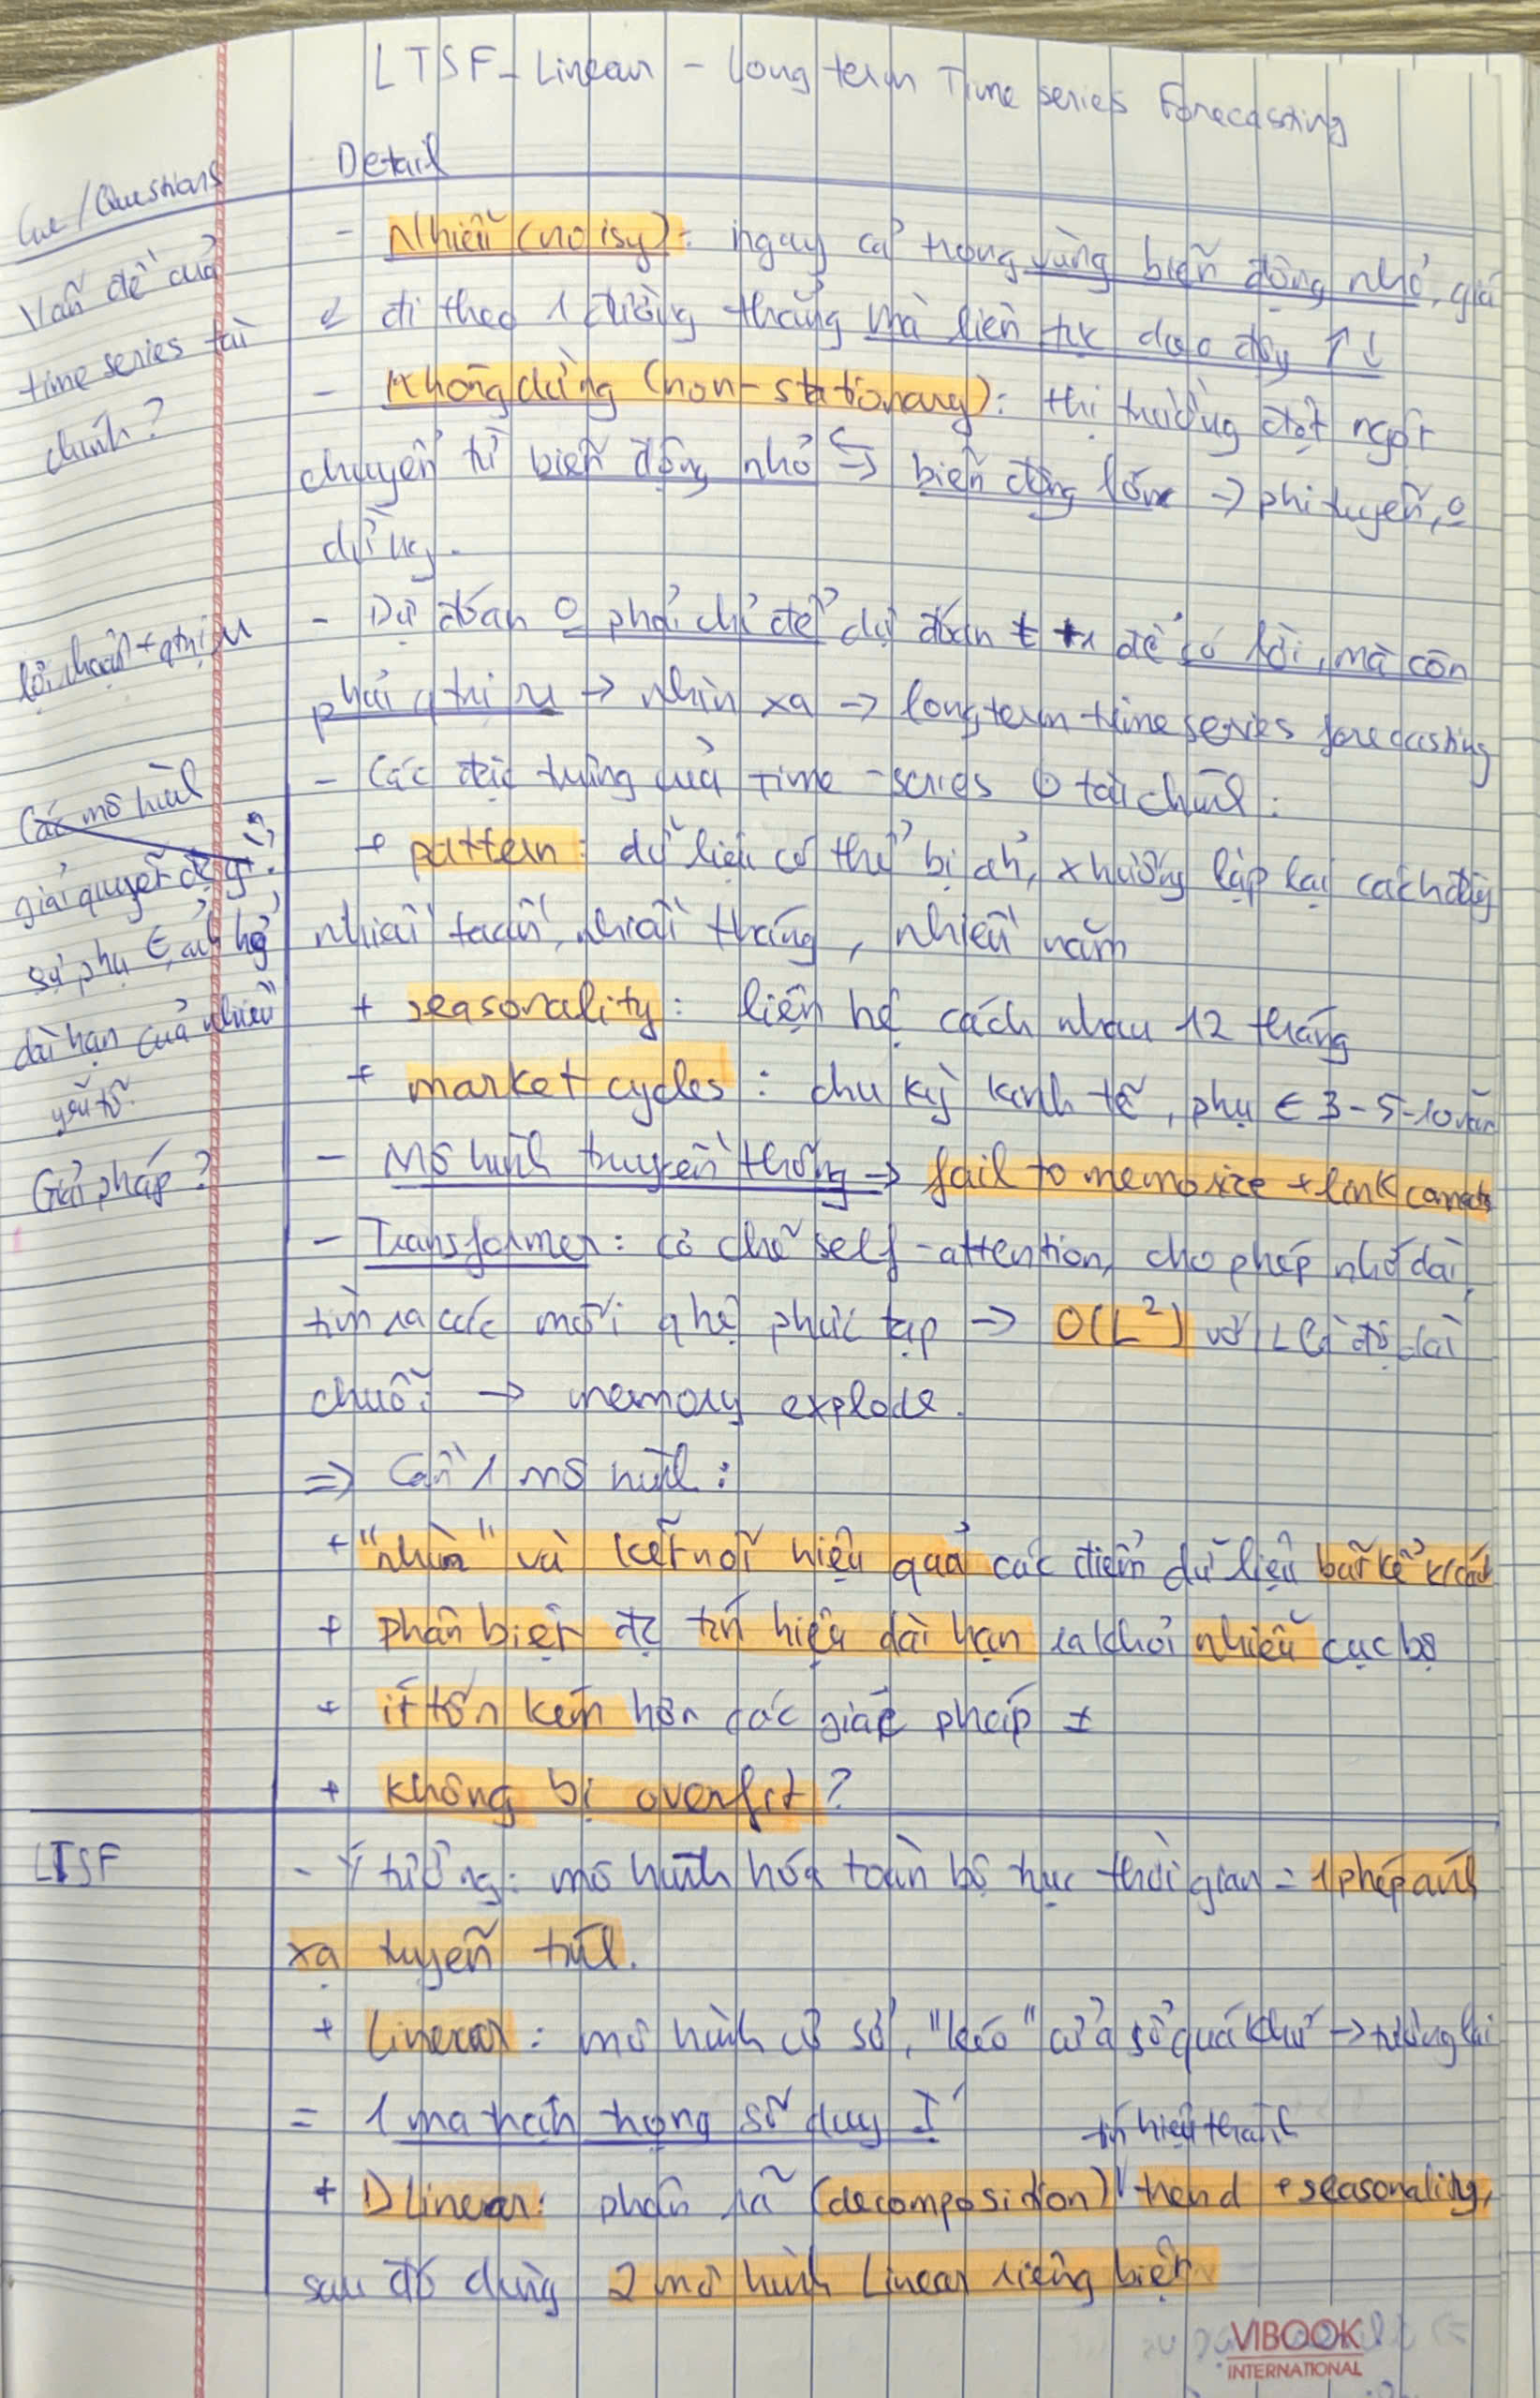
\includegraphics[width=0.92\textwidth,height=0.85\textheight,keepaspectratio]{Figures/note_motivation.jpg}
  \caption{Scan tay --- bối cảnh LTSF / Linear--DLinear (tương ứng Bảng~\ref{tab:cornell-motivation}).}
  \label{fig:scan-motivation}
\end{figure}

\begin{figure}[H]
  \centering
  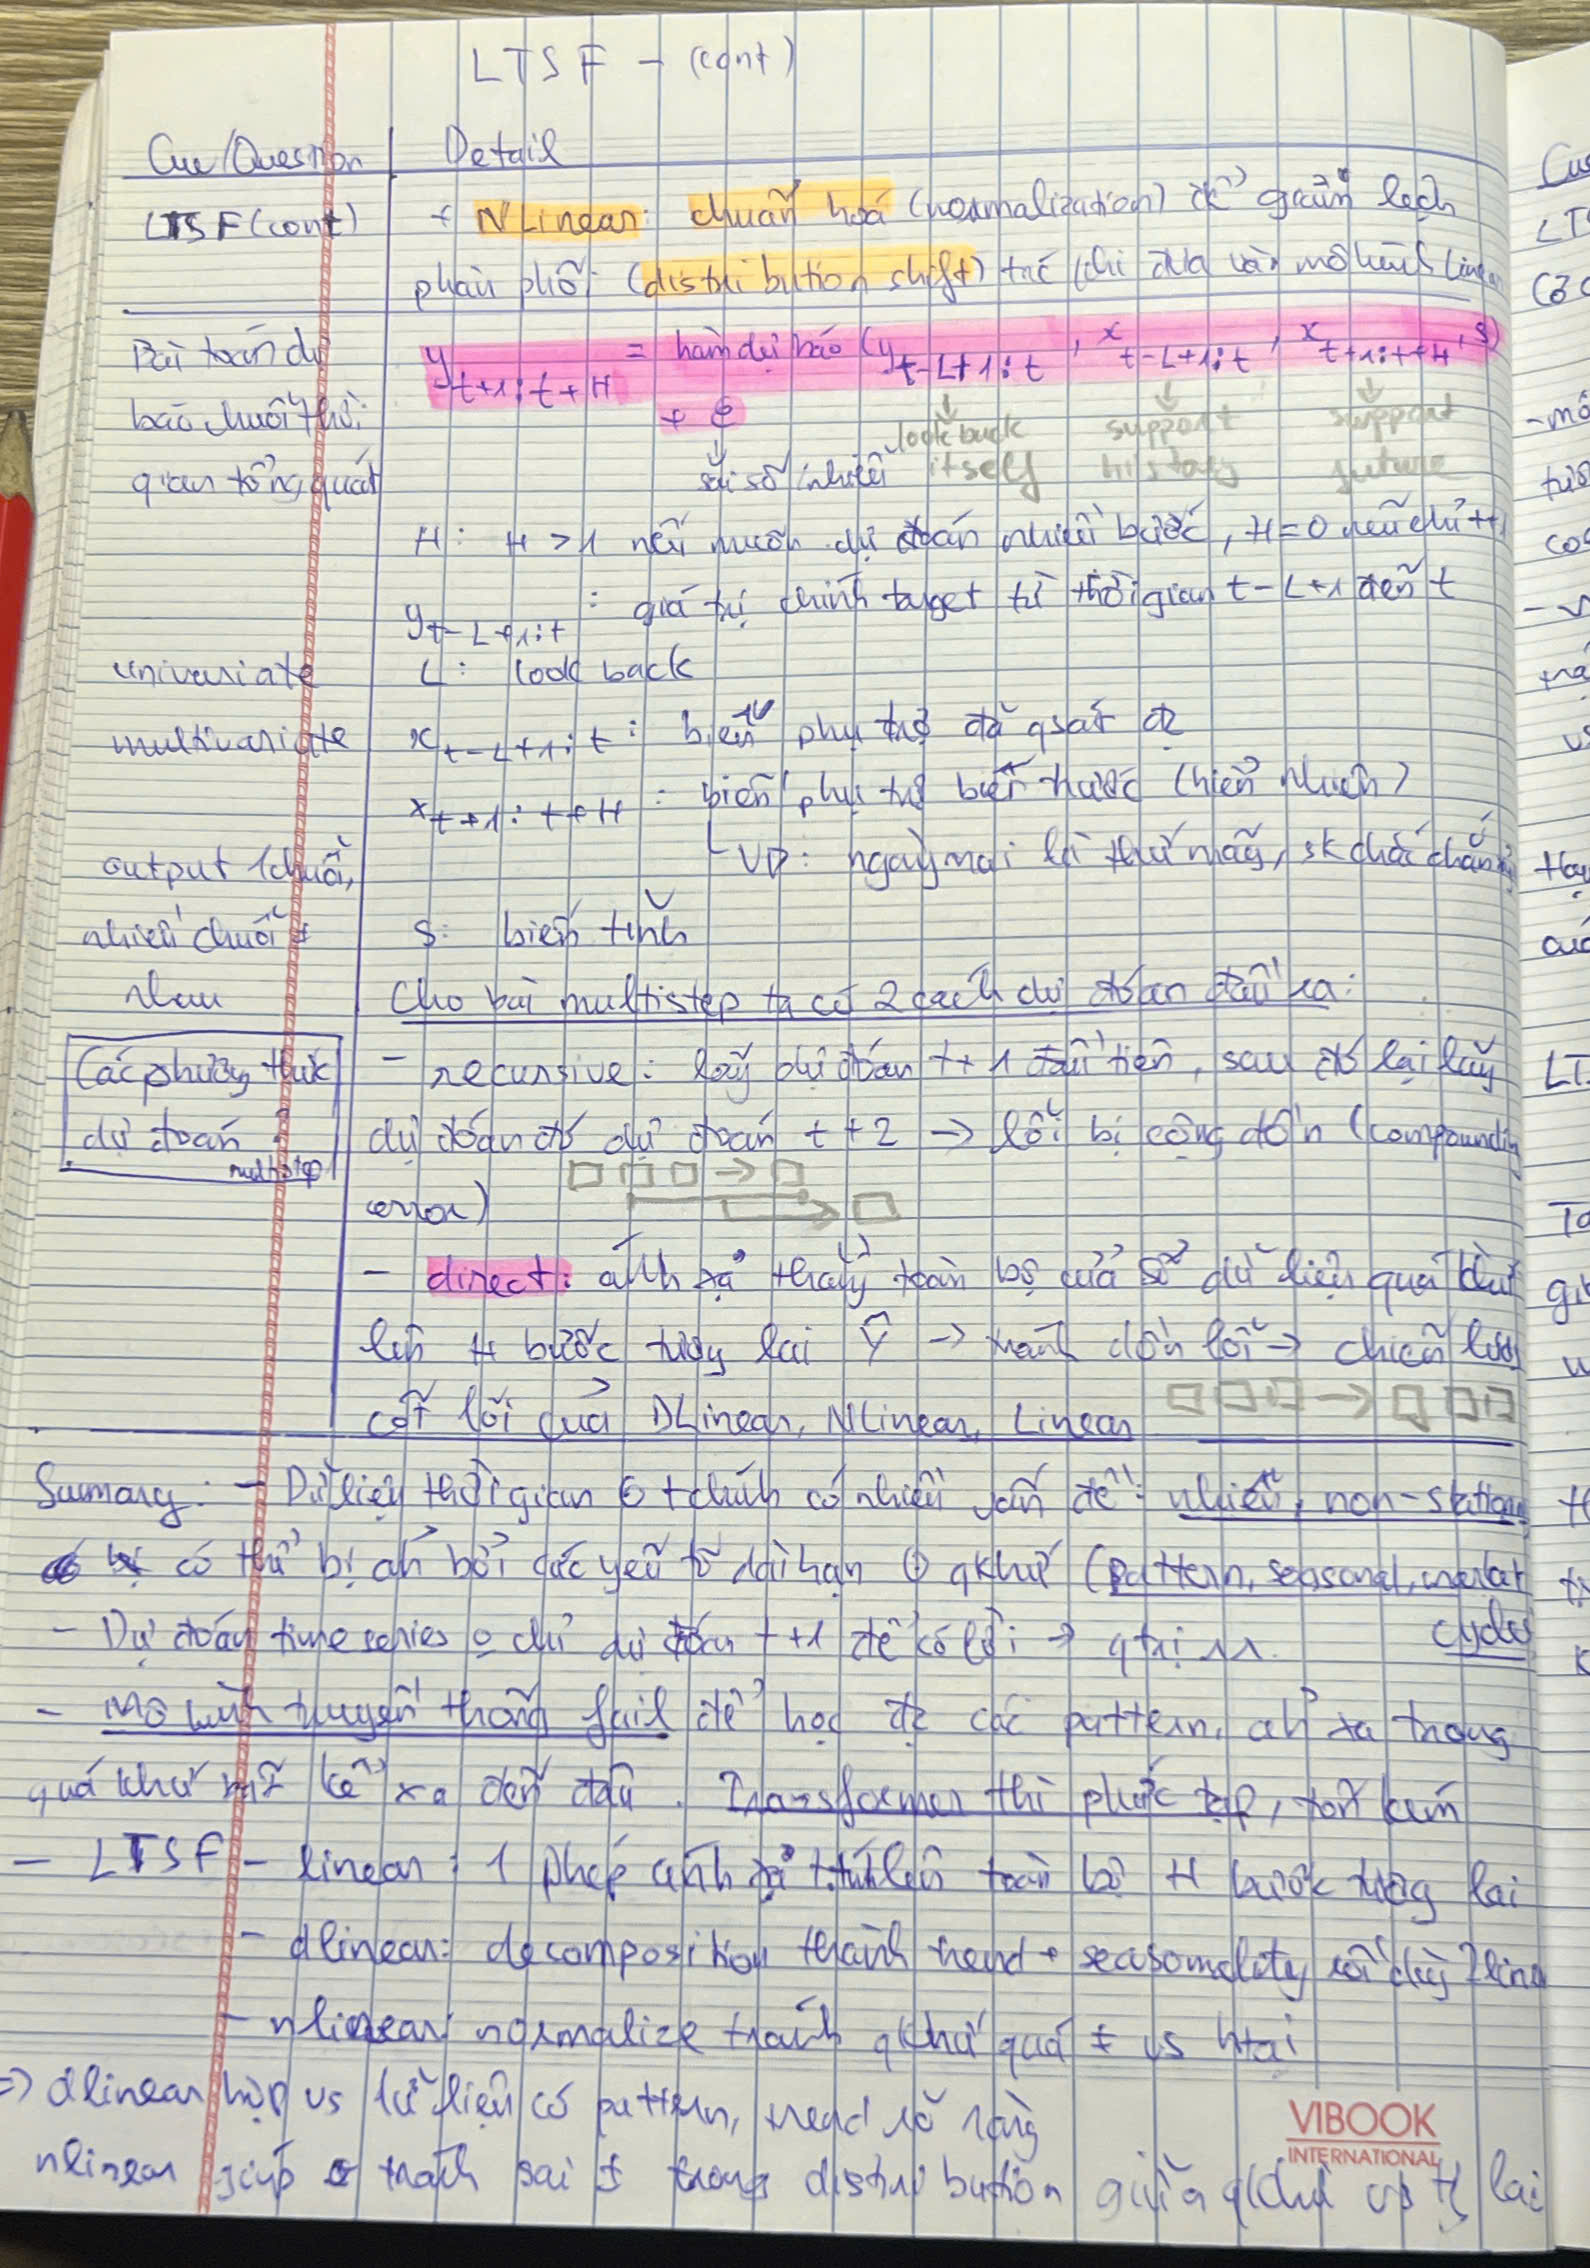
\includegraphics[width=0.92\textwidth,height=0.85\textheight,keepaspectratio]{Figures/note_dms_summary.jpg}
  \caption{Scan tay --- DMS / recursive vs.\ direct (tương ứng Bảng~\ref{tab:cornell-dms}).}
  \label{fig:scan-dms}
\end{figure}

\begin{figure}[H]
  \centering
  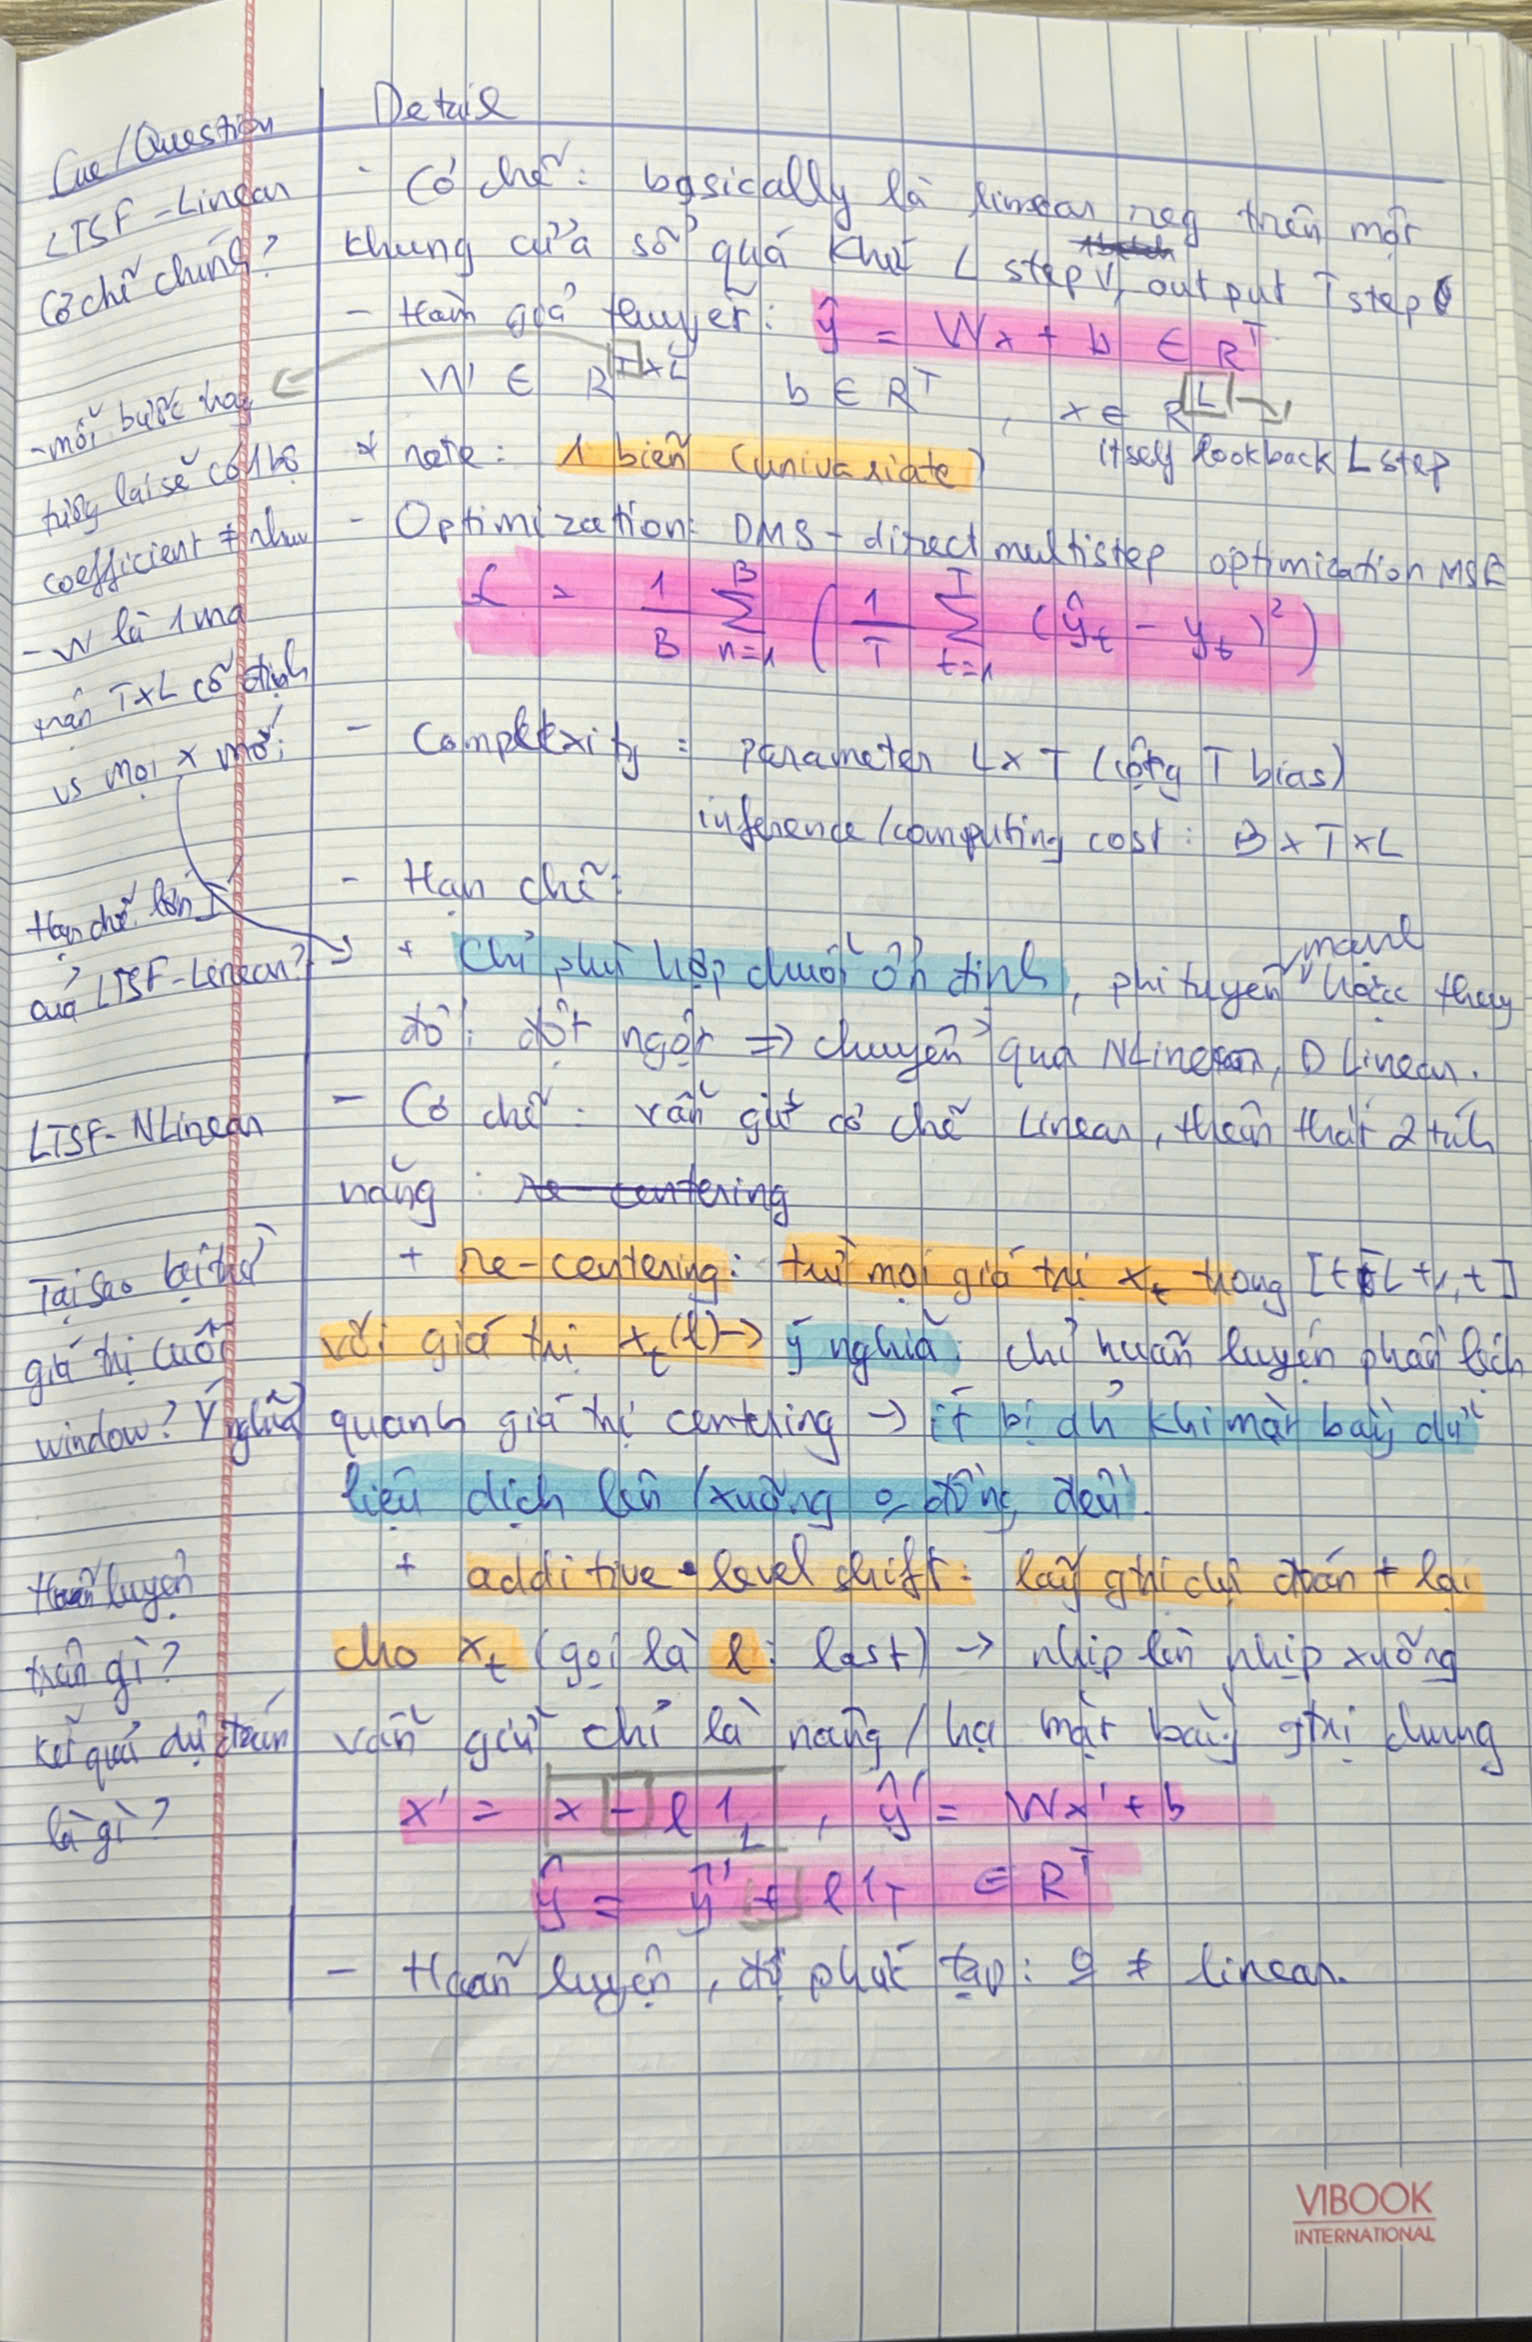
\includegraphics[width=0.92\textwidth,height=0.85\textheight,keepaspectratio]{Figures/note_linear_nlinear.jpg}
  \caption{Scan tay --- Linear \& NLinear (tương ứng Bảng~\ref{tab:cornell-linear-nlinear}).}
  \label{fig:scan-linear-nlinear}
\end{figure}

\begin{figure}[H]
  \centering
  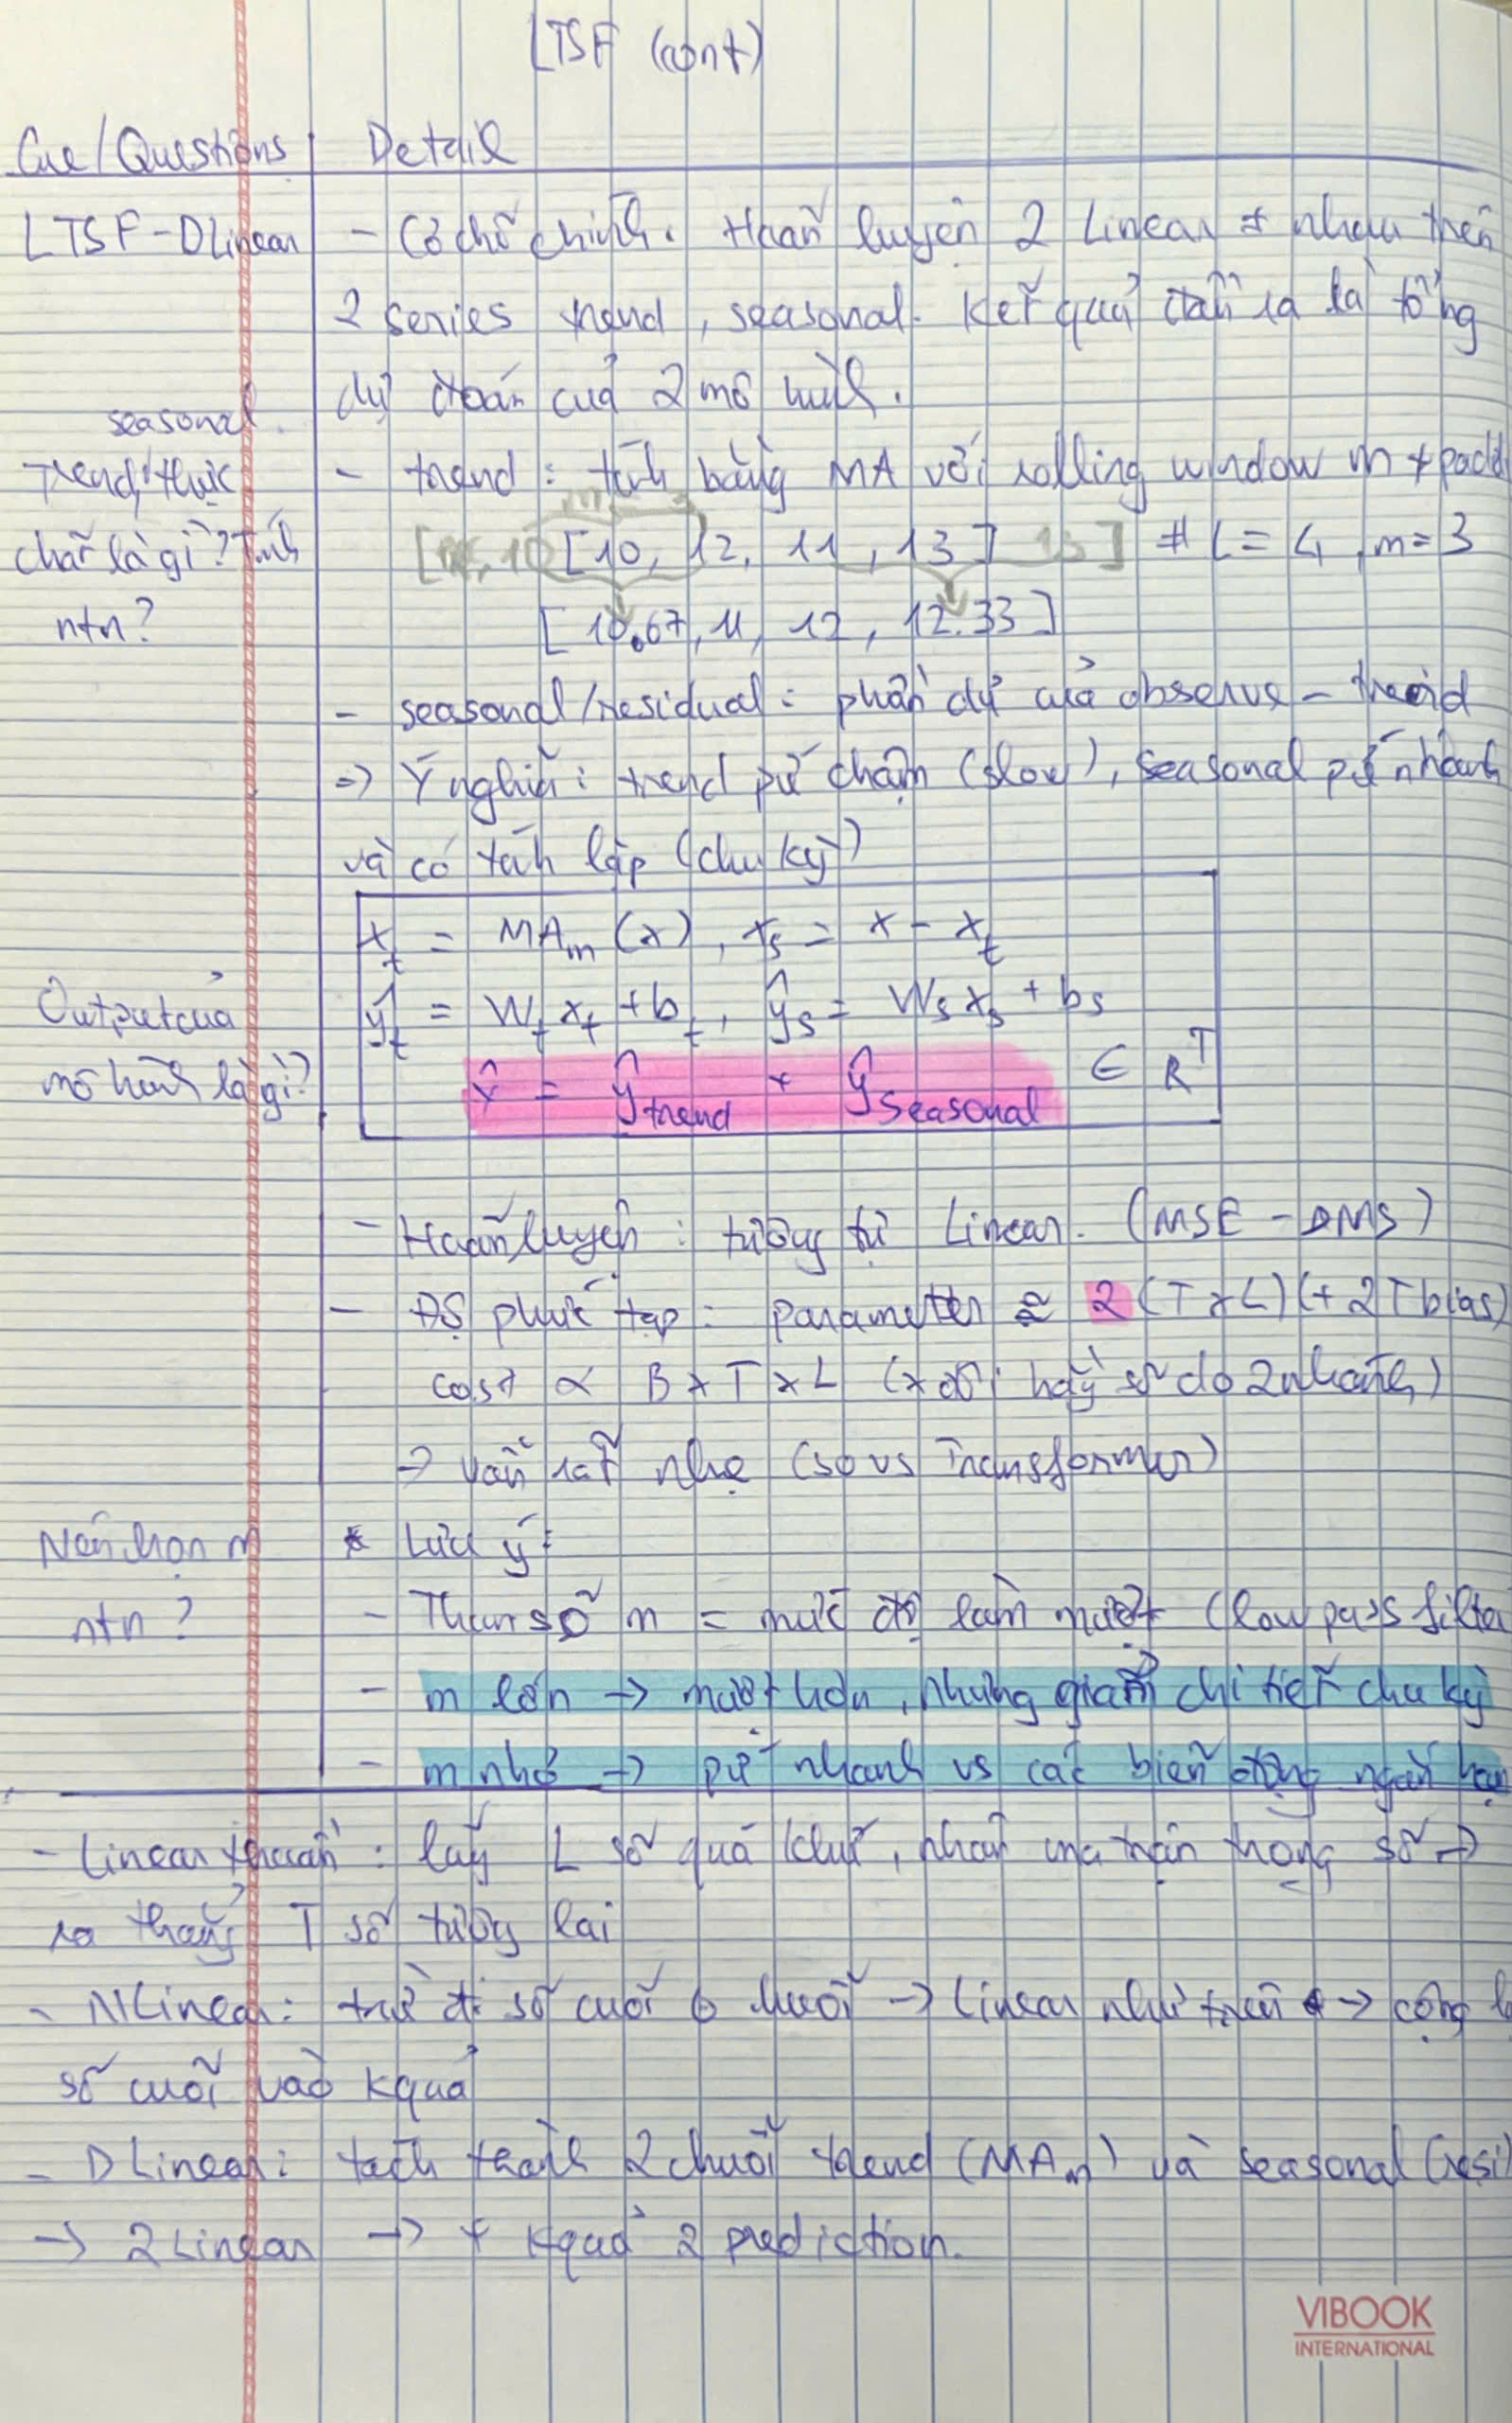
\includegraphics[width=0.92\textwidth,height=0.85\textheight,keepaspectratio]{Figures/note_dlinear.jpg}
  \caption{Scan tay --- DLinear (tương ứng Bảng~\ref{tab:cornell-dlinear}).}
  \label{fig:scan-dlinear}
\end{figure}

\end{document}
